\documentclass[tikz,border=2pt]{standalone}
% Preámbulo común de los diagramas TikZ (misma paleta y letra que las notas)
\usepackage[T1]{fontenc}\usepackage[utf8]{inputenc}
\usepackage{libertinus}\usepackage{libertinust1math}
\usepackage[defaultsans,scale=0.92]{lato}
\usepackage{amsmath,amssymb,bm}
\usepackage{tikz}\usetikzlibrary{calc,positioning,arrows.meta,shapes.geometric,decorations.pathreplacing,decorations.pathmorphing,fit,backgrounds}
\definecolor{snlazul}{HTML}{1E5AA8}\definecolor{snlnoche}{HTML}{14213D}\definecolor{snlvioleta}{HTML}{6C4AB6}
\definecolor{snlcoral}{HTML}{D1495B}\definecolor{snlambar}{HTML}{E09F3E}\definecolor{snlverde}{HTML}{2A9D8F}
\definecolor{snlteal}{HTML}{0F7173}\definecolor{snlgris}{HTML}{5C677D}\definecolor{snlfondo}{HTML}{F4F6FA}
\tikzset{>={Stealth[length=2.2mm]},
  bloque/.style={draw=#1,fill=#1!8,thick,rounded corners=2pt,minimum height=11mm,minimum width=20mm,align=center,font=\small},
  bloque/.default=snlazul,
  suma/.style={draw=snlnoche,thick,circle,inner sep=0pt,minimum size=5mm},
  flecha/.style={->,thick,draw=snlnoche},
  etq/.style={font=\small,text=snlnoche},
  nota/.style={font=\footnotesize\sffamily,text=snlgris,align=center}}

\begin{document}
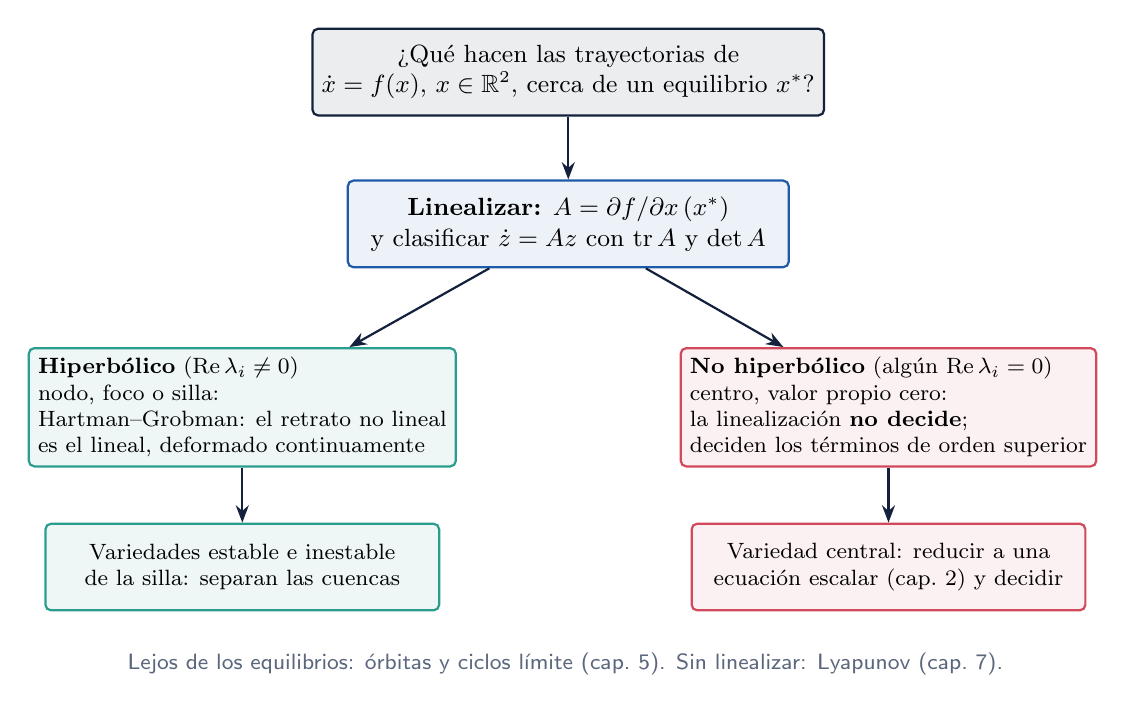
\begin{tikzpicture}[node distance=6mm and 8mm]
 \node[bloque=snlnoche,minimum width=56mm] (q) {¿Qué hacen las trayectorias de\\ $\dot x=f(x)$, $x\in\mathbb R^2$, cerca de un equilibrio $x^*$?};
 \node[bloque=snlazul,below=8mm of q,minimum width=56mm] (lin) {\textbf{Linealizar:} $A=\partial f/\partial x\,(x^*)$\\ y clasificar $\dot z=Az$ con $\operatorname{tr}A$ y $\det A$};
 \node[bloque=snlverde,below left=10mm and -14mm of lin,minimum width=50mm,align=left,font=\footnotesize] (hip) {\textbf{Hiperbólico} ($\operatorname{Re}\lambda_i\neq0$)\\ nodo, foco o silla:\\ Hartman--Grobman: el retrato no lineal\\ es el lineal, deformado continuamente};
 \node[bloque=snlcoral,below right=10mm and -14mm of lin,minimum width=50mm,align=left,font=\footnotesize] (nohip) {\textbf{No hiperbólico} (algún $\operatorname{Re}\lambda_i=0$)\\ centro, valor propio cero:\\ la linealización \textbf{no decide};\\ deciden los términos de orden superior};
 \node[bloque=snlverde,below=7mm of hip,minimum width=50mm,font=\footnotesize] (var) {Variedades estable e inestable\\ de la silla: separan las cuencas};
 \node[bloque=snlcoral,below=7mm of nohip,minimum width=50mm,font=\footnotesize] (cen) {Variedad central: reducir a una\\ ecuación escalar (cap.~2) y decidir};
 \draw[flecha] (q) -- (lin); \draw[flecha] (lin) -- (hip); \draw[flecha] (lin) -- (nohip);
 \draw[flecha] (hip) -- (var); \draw[flecha] (nohip) -- (cen);
 \node[nota,below=4mm of $(var.south)!0.5!(cen.south)$] {Lejos de los equilibrios: órbitas y ciclos límite (cap.~5). Sin linealizar: Lyapunov (cap.~7).};
\end{tikzpicture}
\end{document}
